\section{Experiments}
% In this section, we evaluate our proposed method on the standard DG benchmarks. We first describe the experimental settings, and compare \method{} with state-of-the-art DG methods. We also provide analysis of \method{} 

% \subsection{Evaluation protocols and implementation details}
\subsection{Experiment setups and implementation details}

% \subsubsection{Benchmark datasets.} 
% Following the previous DG studies \cite{cha2021swad,gulrajani2020domainbed}, we evaluate the proposed method on the five benchmark datasets, namely \data{PACS}~\cite{li2017pacs} (4 domains, 7 classes, and $9,991$ examples), \data{VLCS}~\cite{fang2013vlcs} (4 domains, 5 classes, and $10,729$ examples), \data{OfficeHome}~\cite{venkateswara2017officehome} (4 domains, 65 classes, and $15,588$ images), \data{TerraIncognita}~\cite{beery2018terraincognita} (4 domains, 10 classes, and $24,788$ examples), and \data{DomainNet}~\cite{peng2019domainnet} (6 domains, 345 classes, and $586,575$ examples).

% hmm....
\subsubsection{Evaluation protocols and datasets.} 
%We employ DomainBed evaluation protocols~\cite{gulrajani2020domainbed} for fair comparison, with following modifications from \citet{cha2021swad}. 
%\citet{cha2021swad} slightly modifies the protocols by increasing the total training steps for convergence and reducing hyperparameter (HP) search space for efficiency.
% We use DomainBed~\cite{gulrajani2020domainbed} as the testbed for DG tasks. Since the original DomainBed requires very heavy computation resources, we apply minor modifications by increasing total training steps and reducing hyperparameter search space, following Cha \etal \cite{cha2021swad}.
% We evaluate the proposed method in DomainBed comparison protocol  \cite{gulrajani2020domainbed, cha2021swad}.
We employ DomainBed evaluation protocols \cite{gulrajani2020domainbed, cha2021swad} for a fair comparison. The five benchmark datasets are used: \data{PACS}~\cite{li2017pacs} (4 domains, 7 classes, and $9,991$ images), \data{VLCS}~\cite{fang2013vlcs} (4 domains, 5 classes, and $10,729$ images), \data{OfficeHome}~\cite{venkateswara2017officehome} (4 domains, 65 classes, and $15,588$ images), \data{TerraIncognita}~\cite{beery2018terraincognita} (4 domains, 10 classes, and $24,788$ images), and \data{DomainNet}~\cite{peng2019domainnet} (6 domains, 345 classes, and $586,575$ images).
%Details are given in Appendix.
%Performance on each dataset is evaluated by \textit{leave-one-out cross-validation}, where averaged accuracy over all target domains is recorded as a performance of the dataset. When a domain is selected as a target domain, the other domains are used for training. The data in the training domains are splitted again to $80\%$ for training and $20\%$ for validation. Since the out-of-domain performance has rather higher variance than in-domain performance, every experiment is repeated three times by different trial seeds. We report the average score of the three repeated trials.
All performance scores are evaluated by \textit{leave-one-out cross-validation}, where averaging all cases that use a single domain as the target (test) domain and the others as the source (training) domains. Every experiment is repeated three times. We leave 20\% of source domain data for validation. We use training-domain validation for the model selection and the hyperparameter search following DomainBed \cite{gulrajani2020domainbed}.
% The data in the source domains are split again to $80\%$ for training and $20\%$ for validation. 
% Every experiment is repeated three times by different trial seeds. 

\subsubsection{Implementation details.}
We use ResNet-50 \cite{he2016_cvpr_resnet} pre-trained in the ImageNet \cite{russakovsky2015imagenet} as default. The model is optimized using Adam \cite{kingma2015adam} optimizer. A mini-batch contains all domains and 32 examples per domain.
% Proposed method introduces only one hyperparameter $\lambda$. 
The regularization coefficient $\lambda$ is tuned in [1.0, 0.1, 0.01, 0.001].
%using training-domain validation set following DomainBed \cite{gulrajani2020domainbed}. 
The other hyperparameters, such as batch size, learning rate, dropout rate, and weight decay, are tuned in the similar search space proposed in Cha \etal \cite{cha2021swad}. We provide full details in Appendix \ref{sec:additional_impl_details}.

% \subsubsection{Implementation details.}

% \subsubsection{Design of the mean and variance encoders.} 
% We consider the task shift from the pre-trained task in designing encoders. Since high-level representations include task-related semantic information, our encoder adopts multi-scale structure, to utilize diverse representations from low-level to high-level. Instead, we employ as simple as possible architectures, identity function for the mean encoder and bias-only model for the variance encoder, to minimize additional computational cost from the multi-scale design. We also tested architectures with more parameters, but they only increase computational cost without performance improvement.

% \subsubsection{Hyperparameter tuning.} 

\subsection{Main results}

\begin{table}
\centering
\small
\caption{\small {\bf Comparison with domain generalization methods.} Out-of-domain accuracies on five domain generalization benchmarks are shown. 
We highlight the \textbf{best results} in bold. 
The results marked by $\dagger, \ddagger$ are the reported numbers from Gulrajani and Lopez-Paz \cite{gulrajani2020domainbed} and Cha \etal \cite{cha2021swad}, respectively. The results of Fish, SelfReg, and mDSDI are the reported ones from each paper. Average accuracies and standard errors are reported from three trials.
}
\label{table:main_table}
\renewcommand{\arraystretch}{1.1}
\setlength{\tabcolsep}{3pt}
\setlength{\abovetopsep}{0.5em}
\begin{tabular}{l|ccccc|c}
\toprule
\textbf{Algorithm} & \data{PACS}          & \data{VLCS}          & \data{OfficeHome}    & \data{TerraInc}      & \data{DomainNet}     & {Avg.}  \\
\midrule
MMD$^\dagger$ \cite{li2018mmd}                  & 84.7\scriptsize{$\pm0.5$}          & 77.5\scriptsize{$\pm0.9$}          & 66.3\scriptsize{$\pm0.1$}          & 42.2\scriptsize{$\pm1.6$}          & 23.4\scriptsize{$\pm9.5$}          & 58.8           \\
Mixstyle$^\ddagger$ \cite{zhou2021mixstyle}     & 85.2\scriptsize{$\pm0.3$}          & 77.9\scriptsize{$\pm0.5$}          & 60.4\scriptsize{$\pm0.3$}          & 44.0\scriptsize{$\pm0.7$}          & 34.0\scriptsize{$\pm0.1$}          & 60.3           \\
GroupDRO$^\dagger$ \cite{Sagawa2020GroupDRO}    & 84.4\scriptsize{$\pm0.8$}          & 76.7\scriptsize{$\pm0.6$}          & 66.0\scriptsize{$\pm0.7$}          & 43.2\scriptsize{$\pm1.1$}          & 33.3\scriptsize{$\pm0.2$}          & 60.7           \\
IRM$^\dagger$ \cite{arjovsky2019irm}            & 83.5\scriptsize{$\pm0.8$}          & 78.5\scriptsize{$\pm0.5$}          & 64.3\scriptsize{$\pm2.2$}          & 47.6\scriptsize{$\pm0.8$}          & 33.9\scriptsize{$\pm2.8$}          & 61.6           \\
ARM$^\dagger$ \cite{zhang2020arm}               & 85.1\scriptsize{$\pm0.4$}          & 77.6\scriptsize{$\pm0.3$}          & 64.8\scriptsize{$\pm0.3$}          & 45.5\scriptsize{$\pm0.3$}          & 35.5\scriptsize{$\pm0.2$}          & 61.7           \\
VREx$^\dagger$ \cite{krueger2020vrex}           & 84.9\scriptsize{$\pm0.6$}          & 78.3\scriptsize{$\pm0.2$}          & 66.4\scriptsize{$\pm0.6$}          & 46.4\scriptsize{$\pm0.6$}          & 33.6\scriptsize{$\pm2.9$}          & 61.9           \\
CDANN$^\dagger$ \cite{li2018cdann}              & 82.6\scriptsize{$\pm0.9$}          & 77.5\scriptsize{$\pm0.1$}          & 65.8\scriptsize{$\pm1.3$}          & 45.8\scriptsize{$\pm1.6$}          & 38.3\scriptsize{$\pm0.3$}          & 62.0           \\
DANN$^\dagger$ \cite{ganin2016dann}             & 83.6\scriptsize{$\pm0.4$}          & 78.6\scriptsize{$\pm0.4$}          & 65.9\scriptsize{$\pm0.6$}          & 46.7\scriptsize{$\pm0.5$}          & 38.3\scriptsize{$\pm0.1$}          & 62.6           \\
RSC$^\dagger$ \cite{huang2020rsc}               & 85.2\scriptsize{$\pm0.9$}          & 77.1\scriptsize{$\pm0.5$}          & 65.5\scriptsize{$\pm0.9$}          & 46.6\scriptsize{$\pm1.0$}          & 38.9\scriptsize{$\pm0.5$}          & 62.7           \\
MTL$^\dagger$ \cite{blanchard2021mtl_marginal_transfer_learning}    & 84.6\scriptsize{$\pm0.5$}          & 77.2\scriptsize{$\pm0.4$}          & 66.4\scriptsize{$\pm0.5$}          & 45.6\scriptsize{$\pm1.2$}          & 40.6\scriptsize{$\pm0.1$}          & 62.9           \\
Mixup$^\dagger$ \cite{xu2020interdomain_mixup_aaai,yan2020interdomain_mixup,wang2020interdomain_mixup_icassp_dg}             & 84.6\scriptsize{$\pm0.6$}          & 77.4\scriptsize{$\pm0.6$}          & 68.1\scriptsize{$\pm0.3$}          & 47.9\scriptsize{$\pm0.8$}          & 39.2\scriptsize{$\pm0.1$}          & 63.4           \\
MLDG$^\dagger$ \cite{li2018mldg}                & 84.9\scriptsize{$\pm1.0$}          & 77.2\scriptsize{$\pm0.4$}          & 66.8\scriptsize{$\pm0.6$}          & 47.7\scriptsize{$\pm0.9$}          & 41.2\scriptsize{$\pm0.1$}          & 63.6           \\
Fish \cite{shi2022gradient}                     & 85.5\scriptsize{$\pm0.3$}          & 77.8\scriptsize{$\pm0.3$}          & 68.6\scriptsize{$\pm0.4$}          & 45.1\scriptsize{$\pm1.3$}          & 42.7\scriptsize{$\pm0.2$}          & 63.9           \\ 
ERM$^\ddagger$ \cite{vapnik1998statistical}     & 84.2\scriptsize{$\pm0.1$}          & 77.3\scriptsize{$\pm0.1$}          & 67.6\scriptsize{$\pm0.2$}          & 47.8\scriptsize{$\pm0.6$}          & 44.0\scriptsize{$\pm0.1$}          & 64.2           \\
SagNet$^\dagger$ \cite{nam2019sagnet}             & \textbf{86.3\scriptsize{$\pm0.2$}} & 77.8\scriptsize{$\pm0.5$}          & 68.1\scriptsize{$\pm0.1$}          & 48.6\scriptsize{$\pm1.0$}          & 40.3\scriptsize{$\pm0.1$}          & 64.2           \\
SelfReg \cite{kim2021selfreg}                   & 85.6\scriptsize{$\pm0.4$}          & 77.8\scriptsize{$\pm0.9$}          & 67.9\scriptsize{$\pm0.7$}          & 47.0\scriptsize{$\pm0.3$}          & 42.8\scriptsize{$\pm0.0$}          & 64.2           \\ 
CORAL$^\dagger$ \cite{sun2016coral}             & 86.2\scriptsize{$\pm0.3$}          & 78.8\scriptsize{$\pm0.6$}          & 68.7\scriptsize{$\pm0.3$}          & 47.6\scriptsize{$\pm1.0$}          & 41.5\scriptsize{$\pm0.1$}          & 64.5           \\
mDSDI \cite{bui2021mdsdi}              & 86.2\scriptsize{$\pm0.2$}          & \textbf{79.0\scriptsize{$\pm0.3$}}          & 69.2\scriptsize{$\pm0.4$}          & 48.1\scriptsize{$\pm1.4$}          & 42.8\scriptsize{$\pm0.1$}          & 65.1           \\ 
\textbf{\method}      & 85.4\scriptsize{$\pm0.4$}          & \textbf{79.0\scriptsize{$\pm0.0$}} & \textbf{70.5\scriptsize{$\pm0.4$}} & \textbf{50.4\scriptsize{$\pm1.1$}} & \textbf{44.3\scriptsize{$\pm0.2$}} & \textbf{65.9}  \\
\midrule
\multicolumn{7}{l}{\textit{Combined with SWAD \cite{cha2021swad}}}   \\
\midrule
ERM + SWAD$^\ddagger$                & 88.1\scriptsize{$\pm0.1$}          & 79.1\scriptsize{$\pm0.1$}          & 70.6\scriptsize{$\pm0.2$}          & 50.0\scriptsize{$\pm0.3$}          & 46.5\scriptsize{$\pm0.1$}          & 66.9           \\
CORAL + SWAD$^\ddagger$              & 88.3\scriptsize{$\pm0.1$}          & 78.9\scriptsize{$\pm0.1$}          & 71.3\scriptsize{$\pm0.1$}          & 51.0\scriptsize{$\pm0.1$}          & 46.8\scriptsize{$\pm0.0$}          & 67.3           \\
\textbf{\method{} + SWAD}            & \textbf{88.4\scriptsize{$\pm0.1$}} & \textbf{79.6\scriptsize{$\pm0.2$}} & \textbf{72.4\scriptsize{$\pm0.1$}} & \textbf{52.9\scriptsize{$\pm0.2$}} & \textbf{47.0\scriptsize{$\pm0.0$}} & \textbf{68.1} \\
\midrule
\multicolumn{7}{l}{\textit{Using RegNetY-16GF backbone with SWAG pre-training \cite{singh2022swag}}}   \\ \midrule
ERM & 89.6\scriptsize{$\pm0.4$}  &  78.6\scriptsize{$\pm0.3$}  &  71.9\scriptsize{$\pm0.6$}  &  51.4\scriptsize{$\pm1.8$}  &  48.5\scriptsize{$\pm0.6$} & 68.0 \\
\textbf{\method}        & \textbf{97.4\scriptsize{$\pm0.2$}}  &  \textbf{79.9\scriptsize{$\pm0.6$}}  &  \textbf{80.4\scriptsize{$\pm0.2$}}  &  \textbf{58.9\scriptsize{$\pm1.3$}}  &  \textbf{53.8\scriptsize{$\pm0.1$}}  &  \textbf{74.1}  \\
\midrule
ERM + SWAD      & 94.7\scriptsize{$\pm0.2$}  &  79.7\scriptsize{$\pm0.2$}  &  80.0\scriptsize{$\pm0.1$}  &  57.9\scriptsize{$\pm0.7$}  &  53.6\scriptsize{$\pm0.6$}  &  73.2  \\
\textbf{\method{} + SWAD}  & \textbf{96.8\scriptsize{$\pm0.2$}}  &  \textbf{81.7\scriptsize{$\pm0.1$}}  &  \textbf{83.3\scriptsize{$\pm0.1$}}  &  \textbf{64.3\scriptsize{$\pm0.3$}}  &  \textbf{60.7\scriptsize{$\pm0.0$}}  &  \textbf{77.3}  \\
\bottomrule
\end{tabular}
\end{table}
\subsubsection{Comparison with domain generalization methods.}
We provide exhaustive out-of-domain performance comparisons on five DG benchmarks in Table~\ref{table:main_table}. 
Compared to ERM, the proposed MI regularization significantly improves performance on every benchmark dataset, resulting in +1.7pp average improvement. 
%(+1.2pp in \pacs, +1.7pp in \vlcs, +2.9pp in \oh, +2.6pp in \tr, and +0.3pp in \dn). 
Compared with the state-of-the-art methods, \method{} achieves the best performances in all benchmarks, except \pacs. 
Especially, \method{} remarkably outperforms previous methods: +1.3pp in \oh{} (mDSDI \cite{bui2021mdsdi}; $69.2\% \rightarrow 70.5\%$) and +1.8pp in \tr{} (SagNet \cite{nam2019sagnet}; $48.6\% \rightarrow 50.4\%$).
%Especially, \method{} remarkably outperforms previous state-of-the-arts: +1.3pp in \oh{} and +1.8pp in \tr{} compared with mDSDI \cite{bui2021mdsdi} and SagNet \cite{nam2019sagnet}, respectively. 
Considering the extensive experiment setup with 5 datasets and 22 target domains, the results demonstrate the effectiveness of \method{} to the diverse visual data types.

The second part of Table~\ref{table:main_table} shows the performance with stochastic weight averaging densely (SWAD)~\cite{cha2021swad}, a state-of-the-art optimizer for DG by seeking flat minima. Since SWAD is an orthogonal direction to \method{}, we also evaluate the combination of \method{} and SWAD.
% The authors show the flatness of solution is important factor for out-of-domain generalizability and propose SWAD to find flat minima by averaging optimization trajectory. Since seeking flat minima is orthogonal direction to most of DG methods, including \method{}, it can be combined with any other method. Therefore, we compare our method in the setup of SWAD combination. 
As shown in the table, the combination of \method{} and SWAD achieves the best performance in all datasets, resulting in +0.8pp average improvement compared to the previous best results. 


In the last part of Table \ref{table:main_table}, we push the limits of the out-of-domain performance by employing a large-scale backbone, RegNetY-16GF pre-trained by SWAG \cite{singh2022swag}; a weakly-supervised pre-trained model using 3.6 billion noisy Instagram images and hashtags. As shown in our previous study on MI with the oracle model, the pre-trained RegNet has higher MI than ImageNet pre-trained ResNet (Figure \ref{fig:mi}). In the experiments, we first observe that the improvement gap by \method{} becomes remarkably large compared to the ResNet pre-trained model (from +1.7pp to +6.1pp). We presume that this significantly large gap originated from the negative effect of naive fine-tuning as observed by previous works \cite{wortsman2021robust, kumar2022iclr_finetuning_distort} and our study (Figure \ref{fig:mi-regnet}). As shown in Figure \ref{fig:mi-regnet}, \method{} keeps MI with the oracle model high, resulting in remarkable performance gains on large-scale models. We further explore the effect of the scalability of pre-trained models in the later section.
Finally, by combining \method{} with RegNet backbone and SWAD, we achieve the best domain generalization results (77.3\%) on our evaluation benchmark.
% SWAG indicates weakly supervised pre-training using 3.6 billions Instagram images and hashtags. 
% In this setup, \method{} with SWAD remarkably improves the performance, +9.3pp in average, from the ERM.


\begin{table}[t]
\centering
\small
\caption{\small {\bf Comparison with various pre-training datasets, methods, and backbones.} We compare the performance changes according to the scale of the dataset, the method, and the backbone architecture of pre-training. ResNet-50 architecture is used as default. \data{OH}, \data{TI}, and \data{DN} indicate \data{OfficeHome}, \data{TerraIncognita}, and \data{DomainNet}, respectively. Every accuracy is averaged over three trials.
}
\label{table:varying_dataset_method_backbone_scale}
\renewcommand{\arraystretch}{1.1}
\setlength{\tabcolsep}{3pt}
\setlength{\abovetopsep}{0.5em}
\begin{tabular}{lll|ccccc|c} 
\toprule
\textbf{Dataset \scriptsize{(size)}} & \textbf{Pre-training}  & \textbf{Alg.} & \data{PACS} & \data{VLCS} & \data{OH} & \data{TI} & \data{DN} & {Avg.}  \\
\midrule\multirow{6}{*}{ImageNet \scriptsize{(1.3M)}}     & \multirow{2}{*}{ERM}   & ERM             & 84.2          & 77.3          & 67.6                & 47.8              & 44.0             & 64.2           \\
                                             &                        & \method         & 85.4          & 79.0          & 70.5                & 50.4              & 44.3             & 65.9 (+1.7)           \\
%\midrule\multirow{2}{*}{ImageNet (1.3M)}    
\cmidrule{2-9}& \multirow{2}{*}{Barlow Twins}                         & ERM             & 78.7          & 77.3          & 57.6                & 36.9              & 41.7             & 58.4           \\
                                    &                                 & \method         & 80.7          & 79.4          & 63.7                & 43.2              & 42.6             & 61.9 (+3.5)           \\
%\multirow{2}{*}{ImageNet (1.3M)}    
\cmidrule{2-9}& \multirow{2}{*}{MoCo v3}                              & ERM             & 86.7          & 77.3          & 61.8                & 49.1              & 43.8             & 63.7           \\
                                    &                                 & \method         & 86.3          & 78.5          & 66.8                & 48.4              & 44.7             & 65.0 (+1.3)           \\
% \midrule\multirow{2}{*}{ImageNet-21k (14M)} & \multirow{2}{*}{Semantic Softmax}    & ERM                & 65.1           \\
%                                     &                                      & \method             & 65.5 (+0.4)           \\
\midrule\multirow{4}{*}{CLIP \scriptsize{(400M)}}        & \multirow{2}{*}{CLIP \scriptsize{(ResNet)}}   & ERM             & 64.3          & 69.8          & 28.2                & 32.9              & 29.5             & 44.9           \\
                                    &                                 & \method         & 76.6          & 78.9          & 59.5                & 49.0              & 42.0             & 61.2 (+16.3)           \\
%\midrule\multirow{2}{*}{CLIP (400M)}
\cmidrule{2-9}& \multirow{2}{*}{CLIP \scriptsize{(ViT)}}              & ERM             & 83.4          & 75.9          & 66.4                & 35.3              & 44.4             & 61.1           \\
                                    &                                 & \method         & 95.6          & 82.2          & 82.5                & 54.3              & 54.0             & 73.7 (+12.6)           \\
\midrule
\multirow{2}{*}{Instagram \scriptsize{(3.6B)}}  & \multirow{2}{*}{SWAG \scriptsize{(RegNet)}} & ERM      & 89.6          & 78.6          & 71.9                & 51.4              & 48.5               & 68.0           \\
                                   &                                             & \method  & 97.4          & 79.9          & 80.4                & 58.9              & 53.8               & 74.1 (+6.1)           \\
\bottomrule
\end{tabular}
\end{table}
% \subsubsection{Robustness and scalability analysis.}
\subsubsection{\method{} with various pre-trained models.} 
In this subsection, we investigate the robustness of the proposed method to the choice of pre-trained models.
In Table~\ref{table:varying_dataset_method_backbone_scale}, we explore the performance changes of \method{} by varying pre-training datasets, methods, and backbones.
From the pre-training method perspective, we examine two image self-supervised pre-training methods (Barlow Twins \cite{zbontar2021barlowtwins} and MoCo v3 \cite{chen2021mocov3}), one image-language self-supervised pre-training method (CLIP \cite{radford2021clip}), and one weakly-supervised pre-training method (SWAG \cite{singh2022swag}), as well as ImageNet supervised pre-training baseline (ImageNet ERM). 
From the pre-training scale perspective, we employ the ImageNet \cite{russakovsky2015imagenet} dataset of 1.3 million examples, the CLIP dataset of 400 million examples, and the Instagram dataset of 3.6 billion examples. 
We use ResNet-50 \cite{he2016_cvpr_resnet} backbone architecture as default, but a bigger model is also used for the large-scale pre-training, such as ViT-B \cite{dosovitskiy2021vit} for CLIP or RegNetY-16GF \cite{radosavovic2020regnet} for SWAG.
% Following scaling laws~\cite{zhai2021scaling}, we also uses bigger model, such as ViT-B~\cite{dosovitskiy2021vit} or RegNetY-16GF~\cite{radosavovic2020regnet}, than ResNet-50~\cite{he2016_cvpr_resnet} for the large-scale pre-training, such as CLIP or IG-3.6B.

As shown in the table, \method{} improves performances compared with the baseline ERM in all experiments. For the ImageNet pre-training, applying \method{} results in performance improvements of +1.7pp, +3.5pp, and +1.3pp for ERM (supervised learning), Barlow Twins, and MoCo v3, respectively. For the large-scale pre-training, such as CLIP and SWAG, \method{} brings larger performance improvements of +16.3pp, +12.6pp, and +6.1pp for CLIP, CLIP-ViT, and SWAG, respectively.
These experiments demonstrate the robustness of the proposed method to the pre-training methods, datasets, and backbone architectures. 

Notably, performance improvements of \method{} are remarkable with large-scale pre-trained models, such as CLIP, CLIP-ViT, and SWAG. This is consistent with our observation in Section~\ref{subsection:mi_with_oracle}.
Our method helps large-scale pre-trained models (in terms of the pre-training dataset size) not to be biased to the training source domains compared to naive fine-tuning. Especially, naive fine-tuning of CLIP-ViT (61.1\%) shows worse out-of-domain performance than fine-tuning ImageNet pre-trained model (64.2\%). 
%However, \method{} can leverage the pre-trained knowledge from CLIP-ViT (73.7\%), resulting in remarkable improvements than the ImageNet pre-trained model (65.9\%) with a significant gap.
In contrast, \method{} can leverage the pre-trained knowledge from CLIP-ViT, resulting in superior performance (73.7\%) compared with the ImageNet pre-trained model (65.9\%).
In our later analysis, we show that the knowledge of large-scale pre-trained models is more beneficial to domain generalization than the knowledge of ImageNet pre-trained models.


\begin{table}[t]
\centering
\small
\caption{\small {\bf Comparison with methods exploiting pre-trained models.} Out-of-domain accuracies on five domain generalization benchmarks are shown. 
% We highlight the \textbf{best results} by bold. 
Average accuracies and standard errors are reported from three trials.
}
\label{table:learning_from_pretrained}
\renewcommand{\arraystretch}{1.1}
\setlength{\tabcolsep}{5pt}
\setlength{\abovetopsep}{0.5em}
\begin{tabular}{l|ccccc|c} 
\toprule
\textbf{Algorithm}  & \data{PACS} & \data{VLCS} & \data{OfficeHome} & \data{TerraInc} & \data{DomainNet} & Avg.  \\
\midrule
CRD \cite{tian2019crd}             & 82.3\scriptsize{$\pm1.0$}  &  76.6\scriptsize{$\pm0.9$}  &  67.6\scriptsize{$\pm0.4$}  &  44.0\scriptsize{$\pm1.9$}  &  42.1\scriptsize{$\pm0.1$}  &  62.5  \\
VID \cite{ahn2019vid}             & 84.9\scriptsize{$\pm0.3$}  &  76.2\scriptsize{$\pm0.2$}  &  64.6\scriptsize{$\pm0.5$}  &  48.3\scriptsize{$\pm1.3$}  &  42.5\scriptsize{$\pm0.1$}  &  63.3  \\
LP-FT \cite{kumar2022iclr_finetuning_distort}             & 84.6\scriptsize{$\pm0.8$}  &  76.7\scriptsize{$\pm1.5$}  &  65.0\scriptsize{$\pm0.2$}  &  47.1\scriptsize{$\pm0.7$}  &  43.0\scriptsize{$\pm0.1$}  &  63.3  \\
L$^2$-SP \cite{xuhong2018l2sp}         & 83.6\scriptsize{$\pm0.3$}  &  78.8\scriptsize{$\pm0.4$}  &  65.0\scriptsize{$\pm0.3$}  &  47.9\scriptsize{$\pm2.1$}  &  42.5\scriptsize{$\pm0.2$}  &  63.6  \\
DELTA \cite{li2019delta}            & 83.1\scriptsize{$\pm1.1$}  &  77.7\scriptsize{$\pm0.4$}  &  68.5\scriptsize{$\pm0.3$}  &  45.7\scriptsize{$\pm0.9$}  &  42.8\scriptsize{$\pm0.1$}  &  63.6  \\
LwF \cite{li2017lwf}            & 83.1\scriptsize{$\pm0.8$}  &  77.2\scriptsize{$\pm0.7$}  &  70.0\scriptsize{$\pm0.2$}  &  49.2\scriptsize{$\pm1.2$}  &  42.7\scriptsize{$\pm0.1$}  &  64.5  \\
% \method            & 86.3 & 78.5 & 70.0       & 50.0           & 43.8      & 65.7  \\
% \textbf{\method}   & \textbf{85.4} & \textbf{79.0} & \textbf{70.5}       & \textbf{50.4}           & \textbf{44.3}      & \textbf{65.9}  \\
\textbf{\method{}}      & \textbf{85.4\scriptsize{$\pm0.4$}} & \textbf{79.0\scriptsize{$\pm0.0$}} & \textbf{70.5\scriptsize{$\pm0.4$}} & \textbf{50.4\scriptsize{$\pm1.1$}} & \textbf{44.3\scriptsize{$\pm0.2$}} & \textbf{65.9}  \\
\bottomrule
\end{tabular}
\end{table}
\subsubsection{Comparison with methods exploiting pre-trained models.}
\label{subsubsection:learning_from_pretrained_exp}
Other DG methods simply employ pre-trained models as weight initialization, while \method{} additionally exploits it in the training process. This is the first approach to exploit pre-trained models in domain generalization, but there are several studies in other fields for different purposes. Table \ref{table:learning_from_pretrained} provides a comparison of the methods applicable to our DG settings. We exclude the methods that require additional information other than pre-trained models (\eg, pre-training datasets) or are restricted to a specific model.
% Although our approach is the first study to exploit the pre-trained model in the training process for domain generalization, there are several studies that utilize the pre-trained model for different purposes. In the transfer learning field, L$^2$-SP \cite{xuhong2018l2sp} and DELTA \cite{li2019delta} are proposed to improve in-domain performance in the fine-tuning scenario. Learning without forgetting (LwF) \cite{li2017lwf} is designed to maintain old task performance when learning new tasks in the continual learning setting. LP-FT \cite{kumar2022iclr_finetuning_distort} shows that fine-tuning distorts the pre-trained features and it inhibits out-of-distribution generalization. They propose a simple baseline to alleviate the distortion, freezing the feature extractor in the early training phase.
As shown in the table, \method{} outperforms the comparison methods with large margins. These results demonstrate the effectiveness of our method design for the out-of-domain generalization.

\subsection{Analysis of \method{}}

\begin{figure}
    \centering
    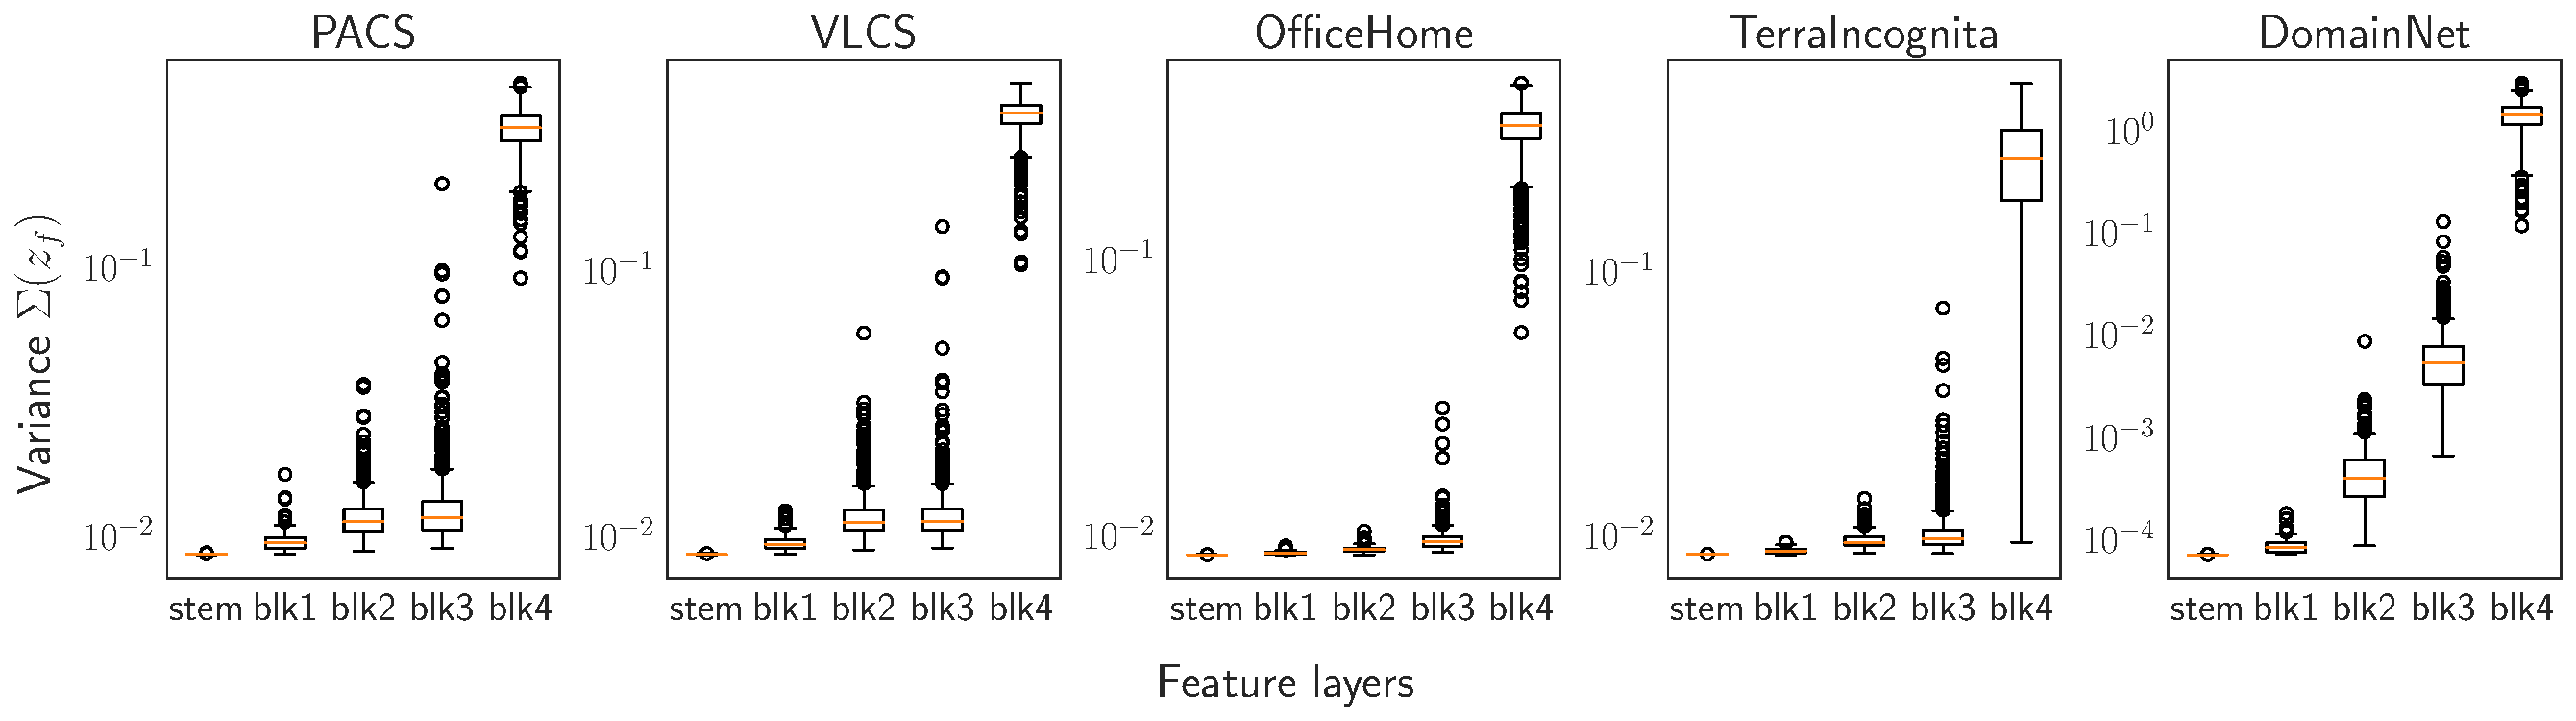
\includegraphics[width=\columnwidth]{figures/sigma_dist_fig.pdf}
    \caption{\small \textbf{Distribution of $\Sigma(z_f)$.} We plot the estimated variances, $\Sigma(z_f)$, for each layer. X-axis indicates the feature layer where the features $z_f$ are collected. In all datasets, the variances increase as the layer is closer to the output.}
    \label{fig:sigma_dist}
\end{figure}
\subsubsection{Loss function interpretation: $\Sigma$ distribution analysis.}
% \subsubsection{$\Sigma$ distribution analysis.}
We can interpret the variance term of \method{}, $\Sigma(z_f)$ in Equation \eqref{eq:method}, as control variables of the distance loss between pre-trained features $z_{f^0}$ and current learning features $z_f$. During the training phase, if the variance values become smaller then the model will preserve MI with the pre-trained model.
% if the model tries to maintain pre-trained information of a certain feature, the variance becomes small. 
On the contrary, when the model needs to learn new information, the variance will increase. We illustrate the learned variances in Figure~\ref{fig:sigma_dist}. The figure shows that pre-trained information is preserved well in lower layers, while task-specific new information is learned in higher layers.
% and the higher the layer, the more new information is learned.
This result is consistent with the interpretation that high layer features represent more task-specific semantic information than low layer features \cite{erhan2009visualizing}; task shifts during fine-tuning make higher layer features learn more semantics than lower layers.
% the widely known understanding that the features of higher layers represent semantic information. 
% Since task shift occurs in the fine-tuning process for DG tasks, the results show that the features of higher layers need to learn new information more than lower layers.


% \begin{figure}[tb]
\begin{center}
\setlength{\tabcolsep}{0pt}
\newcommand\figwidth{.15}
\newcommand\rf{-0.4}
\newcommand\rs{-0.45}
\renewcommand{\arraystretch}{1.3}

\begin{tabular*}{0.8\textwidth}{c @{\extracolsep{\fill}} ccccc}
    \rotatebox[origin=c]{90}{Normal}
    &
    \raisebox{\rf\height}{\includegraphics[width=\figwidth\textwidth]{figures/camelyon_images/T0_H0.png}}
    &
    \raisebox{\rf\height}{\includegraphics[width=\figwidth\textwidth]{figures/camelyon_images/T0_H1.png}}
    &
    \raisebox{\rf\height}{\includegraphics[width=\figwidth\textwidth]{figures/camelyon_images/T0_H2.png}}
    &
    \raisebox{\rf\height}{\includegraphics[width=\figwidth\textwidth]{figures/camelyon_images/T0_H3.png}}
    &
    \raisebox{\rf\height}{\includegraphics[width=\figwidth\textwidth]{figures/camelyon_images/T0_H4.png}}
\\
    \rotatebox[origin=c]{90}{Tumor}
    &
    \raisebox{\rs\height}{\includegraphics[width=\figwidth\textwidth]{figures/camelyon_images/T1_H0.png}}
    &
    \raisebox{\rs\height}{\includegraphics[width=\figwidth\textwidth]{figures/camelyon_images/T1_H1.png}}
    &
    \raisebox{\rs\height}{\includegraphics[width=\figwidth\textwidth]{figures/camelyon_images/T1_H2.png}}
    &
    \raisebox{\rs\height}{\includegraphics[width=\figwidth\textwidth]{figures/camelyon_images/T1_H3.png}}
    &
    \raisebox{\rs\height}{\includegraphics[width=\figwidth\textwidth]{figures/camelyon_images/T1_H4.png}}
\\
    &
    {\small Hospital 1}
    &
    {\small Hospital 2}
    &
    {\small Hospital 3}
    &
    {\small Hospital 4}
    &
    {\small Hospital 5}
\end{tabular*}
%
\end{center}
\caption{\small \textbf{Example images of \data{Camelyon17}.} Distribution shifts between hospitals are caused by the way to acquire and process the tissue slide images.
}
\label{fig:camelyon_examples}
\end{figure}
% %% 2-line examples (2x3)
\begin{figure}
\begin{center}
    \begin{subfigure}{0.4\linewidth}
        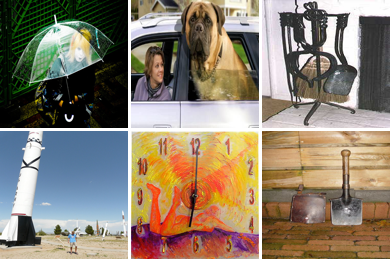
\includegraphics[width=\linewidth]{figures/imagenet_images/2x3grid_IN.png}
        \caption{{ImageNet} (pre-train)}
        \label{fig:imagenet}
    \end{subfigure}
    \quad
    \begin{subfigure}{0.4\linewidth}
        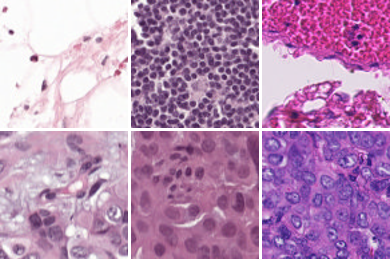
\includegraphics[width=\linewidth]{figures/camelyon_images/2x3grid_CM.png}
        \caption{\data{Camelyon17} (fine-tuning)}
        \label{fig:camelyon}
    \end{subfigure}

    \caption{\small \textbf{Example images of ImageNet and \data{Camelyon17}.} Large distribution shift occurs between pre-training ({ImageNet}) and fine-tuning (\data{Camelyon17}). ImageNet is a multiclass objective recognition task and \data{Camelyon17} is a binary classification task for reading whether the image contains tumor tissue. Instagram-3.6B examples are omitted since it is not publicly available.
    }
    \label{fig:imagenet_camelyon}
\end{center}
\end{figure}

\begin{table}[t]
\centering
\small
\caption{\small {\bf Performance improvements in \data{Camelyon17} medical dataset.} Even in the large distribution shift setup between pre-training and target datasets, \method{} consistently outperforms ERM.
%Bold indicates performance improvement.
Every accuracy is averaged over three trials.}
\label{table:camelyon}
\renewcommand{\arraystretch}{1.1}
\setlength{\tabcolsep}{5pt}
\setlength{\abovetopsep}{0.5em}
\begin{tabular}{ll|ccccc|c} 
\toprule
\textbf{Pretrain}             & \textbf{Algorithm} & 1 & 2 & 3 & 4 & 5 & Avg.  \\
\midrule\multirow{2}{*}{ImageNet ERM}   & ERM                & 97.1      & 94.7      & 95.7      & 96.4      & 90.7      & 94.9  \\
                                        & \method            & {97.5}      & 94.5      & 95.6      & {96.7}      & {93.7}      & {95.6} (+0.7)  \\
\midrule\multirow{2}{*}{SWAG}           & ERM                & 97.0      & 94.1      & 95.3      & 96.0      & 89.5      & 94.4  \\
                                        & \method            & {97.4}      & {95.5}      & {96.5}      & {96.1}      & {90.9}      & {95.3} (+0.9)  \\
\bottomrule
\end{tabular}
\end{table}
\subsubsection{Case study on \data{Camelyon17}: large distribution shift between pre-training and fine-tuning.} As shown in Equation~\eqref{eq:distribution_change}, the tightness of the lower bound is directly connected to the divergence between the representations of oracle and pre-trained models. Therefore, we investigate the case that there is a large shift between pre-trained and target datasets using the medical dataset \cite{bandi2018camelyon17,koh2021wilds}, \data{Camelyon17}. %Among the variants of the dataset, we use the patch-based version provided by Koh \etal \cite{koh2021wilds}. 
This dataset consists of whole-slide images of histological lymph node sections from the five hospitals, where each hospital corresponds to each domain.
% Distribution shifts between hospitals are caused by the way to acquire and process the tissue slide images.
The task is to predict whether the image contains tumor tissue of breast cancer. There is a large gap between the pre-training distribution (ImageNet or Instagram-3.6B) and the fine-tuning distribution (\data{Camelyon17}). Detailed visual examples are provided in Appendix \ref{subsec:imagenet_vs_camelyon17}. The results in Table~\ref{table:camelyon} demonstrate \method{} leads the model to learn robust representations even in the large distribution shift setup between pre-training and fine-tuning.



\begin{figure}
    \centering
    % \begin{subfigure}{\linewidth}
        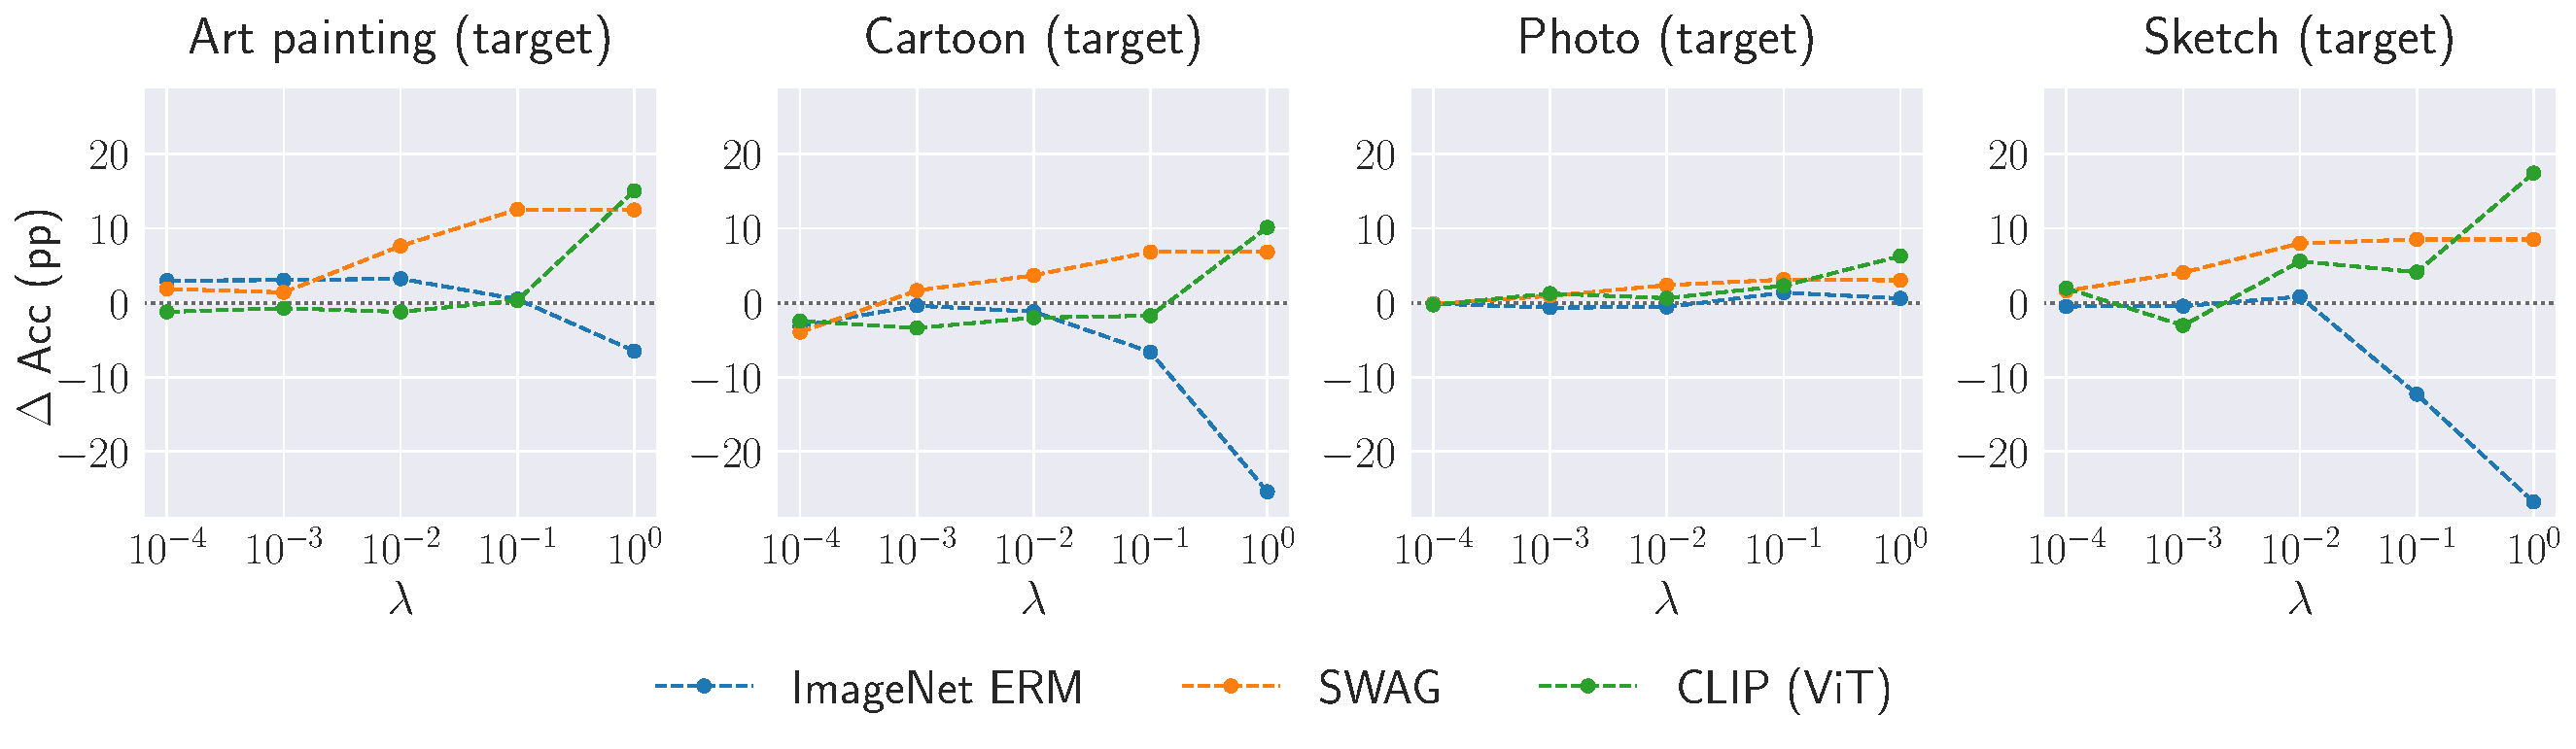
\includegraphics[width=\columnwidth]{figures/accdiff_by_lambda/accdiff_by_lambda_pacs.pdf}
        % \caption{\pacs}
    % \end{subfigure}
    % \begin{subfigure}{0.8\linewidth}
    %     \includegraphics[width=\columnwidth]{figures/accdiff_by_lambda/accdiff_by_lambda_domainnet.pdf}
    %     \caption{\dn}
    % \end{subfigure}
    \caption{\small \textbf{Comparison of three pre-trained models according to $\lambda$.} Y-axis indicates the performance difference of \method{} to ERM. $\lambda$ is the intensity of the mutual information regularization. We compare three models: ResNet-50 pre-trained in ImageNet \cite{he2016_cvpr_resnet}, RegNetY-16GF pre-trained by SWAG \cite{singh2022swag}, and ViT-B pre-trained by CLIP \cite{radford2021clip}.}
    \label{fig:accdiff_varying_lambda}
\end{figure}
\subsubsection{Relationship between the pre-training scale and the intensity of the MI regularization.}
%$\lambda$ is a term representing Lagrangian multiplier $\beta$. 
Our method has a control parameter $\lambda$, which controls the balance between the cross-entropy loss and the MI regularization loss. If $\lambda$ becomes larger, it implies that the strength of MI regularization becomes stronger, while it weakens the strength of the ERM objective. Intuitively, if the pre-trained knowledge is informative enough to the target task, larger $\lambda$ will improve the performances, while if the pre-trained knowledge is uninformative to the target task, then larger $\lambda$ can harm the performances, because of the penalty on the ERM objective.
We compare three pre-trained models (ImageNet pre-trained model, SWAG, and CLIP-ViT) by varying $\lambda$.
Figure~\ref{fig:accdiff_varying_lambda} shows how the out-of-domain performance of \method{} with different pre-trained backbones changes by $\lambda$. The additional results on different datasets are given in Appendix \ref{subsec:accdiff_by_lambda_more}.

First, we observe that the ImageNet pre-trained backbone has a negative correlation between the performance difference and $\lambda$ in target domains. When distribution shifts significantly differ, such as cartoon and sketch domains, we can observe an apparent negative correlation. We presume that it is because the ImageNet samples barely contain non-photo images, such as art painting or sketch images. On the other hand, we observe that \method{} with SWAG and CLIP-ViT backbones make significant performance improvements by choosing larger $\lambda$. In other words, SWAG and CLIP-ViT pre-trained knowledge are helpful to learn robust features for various target domains compared to the ImageNet pre-trained model. Furthermore, it implies that larger pre-trained models trained with massive diverse domain images show less sensitivity to the choice of $\lambda$, not only bringing remarkable performance improvements as shown in Table \ref{table:varying_dataset_method_backbone_scale}.
% It means that the intensity of the regularization should be carefully tuned when using the ImageNet-scale pre-trained backbones. We make a significant performance improvements by tuning $\lambda$ via training-domain validation, but there is still room for improvement depending on how to search the $\lambda$.
% On the other hand, the large-scale pre-trained backbones, such as CLIP and SWAG, the performance is consistently improved as increasing $\lambda$. That is, combining \method{} with large-scale pre-trained backbones not only brings large performance improvements (Table \ref{table:varying_dataset_method_backbone_scale}), but also makes it easy to search appropriate $\lambda$.